\documentclass[border=10pt]{standalone}
\usepackage{tikz}
\usetikzlibrary{arrows.meta,calc}

\begin{document}
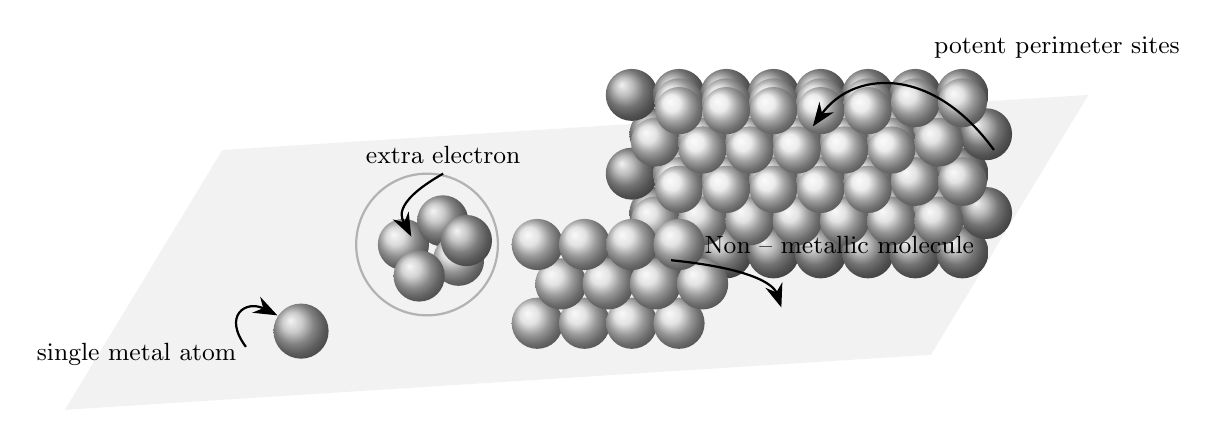
\begin{tikzpicture}[scale=1,
  atom/.style={circle, ball color=#1, shading=ball, minimum size=7mm, inner sep=0pt},
  >=Stealth
]

%------------------------------------------
% Base plane (parallelogram)
%------------------------------------------
\coordinate (A) at (0,0);
\coordinate (B) at (11,0.7);
\coordinate (C) at (13,4);
\coordinate (D) at (2,3.3);

\fill[gray!10] (A)--(B)--(C)--(D)--cycle;

% Helper macro to place spheres in a pseudo‑3D lattice
\newcommand{\cluster}[4]{% (#1,#2)=origin, #3=#rows, #4=#cols
  \pgfmathsetmacro{\ox}{#1}
  \pgfmathsetmacro{\oy}{#2}
  \foreach \i in {0,...,#3}{
    \foreach \j in {0,...,#4}{
      \pgfmathsetmacro{\xx}{\ox + 0.6*\j + 0.3*mod(\i,2)}
      \pgfmathsetmacro{\yy}{\oy + 0.5*\i}
      \node[atom=gray!40] at (\xx,\yy) {};
    }
  }
}

%------------------------------------------
% Large nanoparticle (multi-layer cluster)
%------------------------------------------
% bottom layer (darker rim)
\foreach \i in {0,...,4}{
  \foreach \j in {0,...,7}{
    \pgfmathsetmacro{\xx}{7.2 + 0.6*\j + 0.3*mod(\i,2)}
    \pgfmathsetmacro{\yy}{2 + 0.5*\i}
    % darker at perimeter (i=0 or i=4 or j=0 or j=7)
    \pgfmathsetmacro{\shade}{ifthenelse(\i==0 || \i==4 || \j==0 || \j==7, 70, 40)}
    \node[atom=gray!\shade, minimum size=6.6mm] at (\xx,\yy) {};
  }
}

% second layer
\foreach \i in {0,...,3}{
  \foreach \j in {0,...,6}{
    \pgfmathsetmacro{\xx}{7.5 + 0.6*\j + 0.3*mod(\i,2)}
    \pgfmathsetmacro{\yy}{2.4 + 0.5*\i}
    \node[atom=gray!30, minimum size=6.2mm] at (\xx,\yy) {};
  }
}

% top layer
\foreach \i in {0,...,2}{
  \foreach \j in {0,...,4}{
    \pgfmathsetmacro{\xx}{7.8 + 0.6*\j + 0.3*mod(\i,2)}
    \pgfmathsetmacro{\yy}{2.8 + 0.5*\i}
    \node[atom=gray!20, minimum size=6mm] at (\xx,\yy) {};
  }
}

% Potent perimeter sites label
\draw[-{Stealth[length=3mm]}, thick]
  (11.8,3.3) .. controls (11,4.4) and (10,4.3) .. (9.5,3.6);
\node[align=left] at (12.6,4.6) {\small potent perimeter sites};

%------------------------------------------
% Small non-metallic molecule cluster
%------------------------------------------
\foreach \i in {0,...,2}{
  \foreach \j in {0,...,3}{
    \pgfmathsetmacro{\xx}{6 + 0.6*\j + 0.3*mod(\i,2)}
    \pgfmathsetmacro{\yy}{1.1 + 0.5*\i}
    \node[atom=gray!30, minimum size=6.5mm] at (\xx,\yy) {};
  }
}

% Label for non-metallic molecule
\draw[-{Stealth[length=3mm]}, thick]
  (7.7,1.9) .. controls (8.7,1.8) and (9.0,1.6) .. (9.1,1.3);
\node[anchor=west] at (8.0,2.1) {\small Non -- metallic molecule};

%------------------------------------------
% Cluster with extra electron (inside circle)
%------------------------------------------
\coordinate (Ecenter) at (4.6,2.1);
\node[atom=gray!40, minimum size=6.5mm] at ($(Ecenter)+(-0.3,0)$) {};
\node[atom=gray!55, minimum size=6.5mm] at ($(Ecenter)+(0.2,0.3)$) {};
\node[atom=gray!35, minimum size=6.5mm] at ($(Ecenter)+(0.4,-0.2)$) {};
\node[atom=gray!45, minimum size=6.5mm] at ($(Ecenter)+(-0.1,-0.4)$) {};
\node[atom=gray!60, minimum size=6.5mm] at ($(Ecenter)+(0.5,0.05)$) {};

\draw[thick,gray!60] (Ecenter) circle [radius=0.9];

% Label and arrow for extra electron
\node[anchor=south west] (ee) at (3.7,3.0) {\small extra electron};
\draw[-{Stealth[length=3mm]}, thick]
  (ee.south) .. controls (4.1,2.6) and (4.3,2.4) .. (4.4,2.2);

%------------------------------------------
% Single metal atom
%------------------------------------------
\node[atom=gray!55, minimum size=7mm] (single) at (3,1.0) {};

\draw[-{Stealth[length=3mm]}, thick]
  (2.3,0.8) .. controls (2.0,1.2) and (2.3,1.4) .. (2.7,1.2);
\node[anchor=east] at (2.3,0.7) {\small single metal atom};

\end{tikzpicture}
\end{document}